\chapter{Christologie dans la Chine du VIIIème siècle à travers le Stèle de Xi'an}
\mn{Validation cours Christologie et Culture 2022}
\label{ch:christologieChine}
\section{Introduction}

En 781, à Xi'an, la capitale de l'Empire Tang, fut gravée une stèle présentant la Foi Chrétienne et son développement en Chine, depuis l'arrivée de chrétiens perses 150 ans plus tôt. Notre travail se propose de présenter la façon dont le message chrétien est interrogé par la culture Chinoise de cette époque. Cette inscription est particulièrement pertinente pour une telle étude : 

\begin{quote}
Si les tous premiers textes que nous possédons se contentent de raconter l'histoire du Messie, il fallut bien, un jour en venir à une présentation du message chrétien dans des catégories et des perspectives proprement chinoises. C'est ce que nous fait comprendre le texte de la Stèle de Xi'an composé en 781 [qui] manifeste une vraie synthèse théologique qui puisait dans les trois traditions en présence, christianisme, taoïsme et bouddhisme. \cite[p.~150]{Raguin:JesusMessieXian} 
\end{quote}

Après avoir présenté le contexte culturel et historique de l'écriture de la Stèle, nous étudierons en détail deux passages sur le Christ, pour montrer comment la christologie s'adapte à la culture chinoise, non seulement par la traduction la plus judicieuse possible mais aussi par la mise en avant de certains éléments qui n'étaient pas forcément considérés comme essentiels pour la foi Chrétienne dans d'autres expressions culturelles.
Dans une deuxième partie, nous regarderons les conséquences de ces choix christologiques sur le chemin de salut proposé, à travers l'étude de la section sur les rites et celui sur la \textit{chute}. 

Pour ces deux parties, nous nous appuierons essentiellement sur les travaux de \cite{Havret:stelechretienne} qui propose une traduction et une analyse mot à mot de la Stèle, en développant les références culturelles chinoises des différents passages. De façon complémentaire, Roger-Pol Droit \citep{PolDroit:voyage} propose une réflexion sur les apports de la culture chinoise à la philosophie. Nous ferons régulièrement référence à cette vision synthétique pour éviter une sur-interprétation de tel ou tel passage de la Stèle. 
Enfin, nous partagerons quelques réflexions développées lors de l'élaboration de ce travail, et en particulier la propension qu'ont eut beaucoup de savants étudiant la stèle à penser selon la catégorie d'hérésies.


\section{Contexte et Structure de la Stèle}
 \paragraph{Une culture Chinoise en plein épanouissement.} Si l'empire Tang est souvent présenté comme un « âge d'or » de la civilisation chinoise aussi bien par ses accomplissements militaires que culturels, il le doit à son premier siècle et demi d'existence. Héritière des premiers empires (Qin et Han) ainsi que des évolutions marquées de la période de division, la dynastie Tang est caractérisée par un État très centralisé, dominé politiquement, économiquement et culturellement par sa capitale Chang'an (actuelle Xi'an). C'est là que fut retrouvée la Stèle que nous étudions ici.  
 Initialement très ouvert aux religions étrangères, même s'il soutient officiellement le Taoisme, l'empire se referma en 830-840, soit 50 ans après l'écriture de la Stèle : les mesures de répression des religions étrangères furent prises avec un arrière-fond xénophobe : interdiction de contact entre les Chinois et les étrangers en 836, et interdiction de leurs religions en 845. La présence chrétienne en Chine disparut progressivement, d'autant plus que la source perse perdait de la vitalité du fait de la conquête arabe.
 
\paragraph{Historique de la stèle et de la présence Chrétienne.}
le
premier prêtre nestorien à se présenter à Chang'an fut en 635 un
certain Alopen. Il y fut reçu avec des honneurs dignes d'un ambassadeur. Nous avons conservé la première partie du document qu'il écrivit à la demande de l'empereur  pour présenter la foi chrétienne,  le \textit{livre de Jésus-Messie}. Sa lecture n'est pas un trop grand dépaysement pour un lecteur occidental du XXI\textsuperscript{è} comme le montre ces passages sur la naissance du Christ : 
\begin{quote}
    Le \textit{vent frais} entra dans le corps d'une vierge nommée Mo-yen selon les instructions du Seigneur du Ciel. Soudain, Mo-yen devint enceinte.  \sn{\cite[151]{saeki:nestorianDocumentsChine}, ma traduction de l'Anglais}
\end{quote}
Cette profession de Foi est entrecoupée de commentaires, par exemple : 
\begin{quote}
    Il y eu cependant des personnes ignorantes qui dirent que si la Vierge avait conçu un fils par l'action du \textit{vent Frais} et lui avait donné naissance, alors un tel fils devait être au statut le plus inférieur dans le monde. (157)
\end{quote}
Pour les détromper,
\begin{quote}
     quand \textit{I-shu Mi-Shih-ho} fut né, le monde entier vit des signes brillants au Ciel et sur Terre. Enfin, une nouvelle Étoile apparut dans le ciel  [\ldots] aussi grosse qu'une roue de char, lumineuse et claire au dessus de l'endroit où le Seigneur du Ciel se trouvait (160-162)
\end{quote}
Ce premier témoignage chrétien en Chinois \sn{\cite[p.38]{Raguin:JesusMessieXian}} a été selon toute vraisemblance composé à partir de documents en Syriaque.  
A la suite de ce texte, Alopen put créer un monastère avec 21 moines. 

La stèle qui nous intéresse fut écrite quant à elle 150 ans plus tard, en 781. Elle a été redécouverte au XVII\textsuperscript{e} dans le quartier des marchands de Chang'an, provoquant stupéfaction en Occident. Elle est connue selon de nombreux noms, du fait des différentes prononciations de Chang'an  - alias Si-gnan-Fou alias Xi'an. Par ailleurs, elle est appelée alternativement \textit{inscription nestorienne} (\cite{saeki:nestorianDocumentsChine}) du fait de l'origine syriaque des moines, ou simplement \textit{Stèle Chrétienne}, afin de ne pas projeter sur la stèle la marque des discussions théologiques des premiers conciles, tendance d'autant plus présente que historiquement on a eu tendance à considérer comme hérétique des expressions de foi dans des contextes culturels différents. La stèle présente la foi chrétienne de façon bien différente du texte écrit 150 ans auparavant par Alopen, du fait d'un travail théologique d'acculturation important. 


\paragraph{Une stèle écrite en excellent Chinois, signe d'une compréhension fine de la culture chinoise}. On pense qu'elle fut écrite par le moine perse et évêque de Chine \textit{Adam}. Il fut très probablement aidé dans sa tâche, aidé par un lettré chinois King-tsing\cite[p.~5]{Havret:stelechretienne}.
Ce lettré a d'ailleurs pu être qualifié au début du XIX\textsuperscript{e} comme :
\begin{quote}
    [...] habile mais porté par la secte de \textit{Tao} \sn{P. Gaubil, Mémoires concernant les Chinois, Tom. XVI, 1811, p. 371.}
\end{quote}


\paragraph{Une vraie Christologie en contexte chinois} Par rapport à l'exposé de foi d'Alopen, le texte n'est plus une simple traduction mais une vraie christologie chinoise, reprenant certaines catégories taoistes, culture dominante de l'élite chinoise à l'époque, ou bouddhistes.

\paragraph{Le titre de la Stèle indique le projet d'acculturation}

\begin{figure}[h!]
    \centering
    \sidecaption{Titre de l'inscription \cite{Pauthier:linscriptionSinganfou} Monument (rappelant) la propagation à travers l'Empire du Milieu de l'Illustre (King) Religion du Ta-ts'in}
    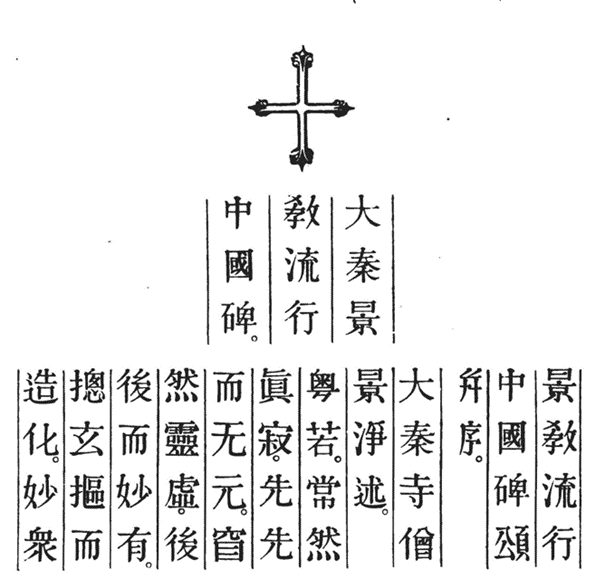
\includegraphics[width=\textwidth]{ChristologieCultureHistoire/Images/PremierParagrapheStele.png}
 
    \label{fig:my_label}
\end{figure}
 Si le livre d'Alopen 150 ans plutôt s'appelait simplement "Sûtra de Jésus-Messiah", le titre de la Stèle est le suivant :
\begin{quote}
    Monument rappelant la propagation à travers l'Empire du Milieu de l'Illustre Religion de Ta-ts'in. \cite{Havret:stelechretienne}
\end{quote}
Ta-ts'in (ou \emph{Da Qin}) indique l'Empire Gréco-Romain. Cette référence peut étonner quand on sait la répugnance des Eglises perses à être trop liées à Byzance. D'ailleurs, traditionnellement, le christianisme en Chine était appelé \textit{Bose Jiao}, l'\textit{enseignement Perse}.  En 745, il prend l'appellation officielle de religion de Da-Qin  possiblement par la chute de l'empire Sassanide perse un siècle plus tôt, qui rend caduque le terme de Perse, l'arrivée d'ambassades byzantines en Chine (attestée en 742) mais aussi par la référence à la philosophie grecque ainsi qu'à l'attribution de voyages en \textit{Da Qin} par le fondateur du Taoisme, Laozi :
\begin{quote}
    Calling Christianity the 'Religion of Da Qin' shows that the Nestorians of the Tang undeniably possessed a sensitive awareness of their political environment within China, and probably internationally as well, and moved with considerable acumen to secure the best possible position for themselves within it (\cite{Barrett:TaoismChristianity})
\end{quote}

\paragraph{Un découpage proposé en 25 sections} La stèle peut être découpée en 25 sections, la première sur les attributs de Dieu, puis les trois suivantes sur la Création et la Chute de l'homme (surtout pour développer l'idée d'un homme bon avant la chute par l'orgueil), puis les deux suivantes sur le Christ. A partir de la section 8, on trouve les caractéristiques de la religion, le baptême, les moines, l'éthique, puis plusieurs sections sur l'histoire des chrétiens en Chine, montrant une loyauté forte vis à vis des autorités politiques chinoises. Nous nous concentrerons sur les premières sections et en particulier les sections 6 et 7 proprement christologiques.  Il faut noter qu'une partie importante est liée à l'histoire du christianisme en Chine et la protection des empereurs. Cette attitude peut être mise en parallèle avec celle des premières communautés chrétiennes, avec Paul, montrant la compatibilité du christianisme avec l'Empire Romain (\cite{Baslez:MondeDevnuChretien}). 






\section{la partie proprement Christologique}

\subsection{Section 6 : l'incarnation} 

La première section qui nous intéresse parle de l'incarnation. Nous indiquerons à chaque fois les deux traductions en Français qui font foi (\cite{Havret:stelechretienne} et \cite{Pauthier:linscriptionSinganfou} \sn{la traduction de Havret est une traduction en latin et français mais la traduction française n'est pas complète - je l'ai complété à partir du texte latin}) :
 
\begin{tabular}{p{0.45\textwidth}p{0.45\textwidth}}
\\
Cependant, notre Trinité s'est comme multipliée, l'illustre et vénérable Messie, voilant et cachant son auguste majesté, se rendant tout semblable aux hommes, est venu en ce monde. les Puissances angéliques publièrent la bonne nouvelle; une femme vierge enfanta le Saint dans la grande Ts'in. Les esprits dans le Ciel annoncèrent la bonne nouvelle : "une Vierge a enfanté le Saint dans la grande Ts'in". Une étoile resplendissante a proclamé la faveur et la Perse, apercevant son éclat, vint lui faire hommage de ses présents. \cite[p. 35]{Havret:stelechretienne} & 

Ce faut alors que notre \textsc{Unité-trine} divisa sa personne dans le resplendissant et vénérable Messie, en voilant sa véritable majesté. il apparut dans le monde comme un simple mortel. Les Esprits dans le ciel annoncèrent la bonne nouvelle : "une Vierge a enfanté le Saint dans la Syrie !"  Une constellation resplendissante a proclamé l'heureux événement; les Perses ayant aperçu sa clarté, sont venus apporter leur tribut. \cite[p. 9]{Pauthier:linscriptionSinganfou} \\
                                                                                  
\end{tabular}
 
 \paragraph{Wo Sanyi, notre "trois-Un". } La pensée Taoiste utilisent le terme de Sanyi :  

\begin{quote} Le terme employé pour désigner la Trinité est un terme taoïste, \emph{sanyi} le "Trois-Un". mais pour signifier qu'il s'agissait de la Trinité Chrétienne, l'auteur de l'inscription a ajusté le caractère "\emph{Wo}" qui signifie "mon/notre". Ainsi le terme taoïste a pris un sens chrétien, "Notre Trois-Un".
    \cite[p.43]{Raguin:JesusMessieXian}
\end{quote}
Quelle est cette trinité taoïste ? Le Trois est pensé comme facteur d'harmonie entre l'Un et le Multiple permettant de «court-circuiter» la référence à Dieu ou à quelque instance supra-cosmique.\cite{Cheng:triadeChinoise}


Le terme utilisé pour le Christ est le terme syriaque de \textit{Messie}, translittéré et non traduit.

 "\textit{Voilant et cachant son auguste majesté, se rendant tout semblable aux hommes, est venu en ce monde}" est quasiment la traduction de Ph 2,6-7, soulignant l'abaissement du Christ.
 

\paragraph{Insistance sur le Ciel et l'environnement}  les cieux (\textit{constellation}) prennent une partie importante dans les deux sections sur le Christ, avec tout un passage sur l'Etoile des mages. On peut  déceler le souhait de l'auteur de montrer ce qu'est le Christ non pas en le décrivant directement comme \textit{forme},  causes ou \textit{logos} mais en insistant sur le \textit{fond},  \textit{le Ciel} qui \textit{ne s'exprime pas}. \cite[p. 109]{PolDroit:voyage} . 
\begin{quote}
    La philosophie gréco-européenne privilégie la « forme » – en grec ancien, \textit{eïdos}. Une « idée » est d’abord une « forme », qui se découpe sur un fond d’espace indifférencié. C’est ce fond d’espace qui retient l’attention chinoise, plutôt que la forme qui s’en détache. Scruter le fond plutôt que les formes, l’indifférencié plutôt que les différences, l’espace plutôt que les choses qui s’y trouvent et s’y découpent, telle pourrait être la première caractéristique de l’attitude chinoise.\cite[pp. 110-111]{PolDroit:voyage}  
\end{quote}
Dès lors, l'attitude des mages perses qui scrutent dans \textit{le Ciel} ce qui change, est finalement celle du sage Chinois. Pour le Taoisme, ce n'est pas par le discours, qui segmente et découpe mais par le biais d'histoires déroutantes, \textit{comme celle de l'étoile des mages}, que l'on peut transmettre la voie. \cite[p. 130-141]{PolDroit:voyage} 
 




\subsection{section 7 : la rédemption } 


Après l'incarnation, le texte développe en plusieurs paragraphes l'action de Jésus : 


\begin{tabular}{p{0.45\textwidth}p{0.45\textwidth}}
\\
Il accomplit les lois anciennes qu'avaient écrites les vingt-quatre Saints, direction des empires dans les conseils. Il fonda la nouvelle religion que la Trine unité, Esprit très pur, n'exprime pas au moyen de paroles, formant à la pratique des vertus par la vraie foi.  & Ainsi, s'est trouvé accompli ce que les vingt-quatre saints avaient annoncée dans l'ancienne loi : " le gouvernement des familles et des États par une grande et suprême doctrine. Il établit la doctrine pure de l'\textsc{unité-trine}, sans l'appeler une nouvelle religion. Il fortifia les bonnes habitudes par l'usage de la vraie foi. \\
\end{tabular}

\paragraph{Jésus est présenté comme un sage} Le texte insiste sur l'Esprit qui soutient la vertu sans passer par une loi (cf Jr 31,33 \sn{Jr 31,33 \textit{Je mettrai ma loi au dedans d'eux, Je l'écrirai dans leur coeur} \newline 2 Co 3,3\textit{Vous êtes manifestement une lettre de Christ, écrite, par notre ministère, non avec de l'encre, mais avec l'Esprit du Dieu vivant, non sur des tables de pierre, mais sur des tables de chair, sur les coeurs.}}  ou encore 2 Co 3,3).

Par cet  \textit{Esprit très pur, qui n'exprime pas au moyen de paroles formant à la pratique des vertus par la vraie foi}, l'auteur propose probablement une théologie accessible à la culture chinoise. pour les Chinois en effet,  ce n'est pas au moyen de raisonnements qu'on atteint le Ciel, qui s'éprouve directement
\cite[p. 117]{PolDroit:voyage} même si notre participation au Ciel en ce monde est parfois voilée.


Cependant, l'auteur ne s'arrête pas à une approche \textit{sans parole} puisqu'il mentionne les \textit{huit béatitudes} : 

\begin{tabular}{p{0.45\textwidth}p{0.45\textwidth}}
\\
Il institua les règles des huit fins, pour purifier les facultés et perfectionner les saints; il ouvrit la porte des trois principes,& Il posa les lois des huit limites morales que l'on ne doit point franchir. la poussière de la terre, purifiée comme le métal dans la fournaise, devint la vérité parfaite. Il enseigna au moindre les trois grandes vertus cardinales; 
\\ 
 en ouvrant les portes la vie et supprimant la mort. & il lui ouvrit les sources de la vie, et anéantit la mort.
\end{tabular}


 \paragraph{Référence à la Bible} Après avoir insisté sur l'éthique de Jésus, l'auteur met l'accent sur le corpus biblique, à la fois dans le registre de l'\textit{accomplissement} de l'Ancien Testament et ses 24 livres/ Saints mentionnés plus haut \sn{hors livres deutérocanoniques} que de l'annonce d'un nouveau Testament\sn{ l'auteur décompte 27 livres alors que le Corpus syriaque ne reconnaissait initialement que 22 livres (l'Apocalypse et les épîtres générales reconnus tardivement) }. 

 \paragraph{Sauver par le registre de la grâce} Face à poussière (Lieu-tch'en), expression bouddhique pour désigner les \textit{souillures de la pureté du coeur},  le texte mentionne les 8 lois morales (Pa-King, "8 circonstances"), comprises comme les Béatitudes (8 béatitudes chez Mt).  Sont aussi mentionnés la porte des trois vertus cardinales (Tch'ang), porte qui ouvre aussi à la vie et supprimant la mort (Mié-se) selon une expression chrétienne traditionnelle. 

Puis suit une expression typiquement bouddhique du soleil lumineux triomphant des porte des enfers (ti-yu) mot à mot \textit{prison de la terre} \cite[p. 49]{Havret:stelechretienne}.  Satan est ici appelé par le terme chinois \textit{Mo}, d'où la traduction de démon :

\begin{tabular}{p{0.45\textwidth}p{0.45\textwidth}}
\\
Il suspendit le soleil lumineux pour triompher de l'empire de ténèbres et {dès lors }les ruses du démons furent toutes pénétrées et déjouées
&  Il suspendit au ciel le brillant soleil de la vérité pour dissiper les habitations des ténèbres; les ruses mensongères du démon furent dès lors pénétrées et déjouées. \\
\end{tabular}



 
 
 

\begin{tabular}{p{0.45\textwidth}p{0.45\textwidth}}
\\
Conduisant à la rame la barque de la miséricorde, il s'éleva aux demeures lumineuses; dès lors quiconque possède une âme a trouvé son salut. L'oeuvre de la toute puissance étant ainsi consommée, il monta en plein midi, homme déifié.& Il mit en mouvement le navire de la miséricorde pour s'élever aux brillantes demeures; les âmes qu'il renfermait purent dès lors, en traversant le fleuve de la vie, obtenir cette fin glorieuse. A l'heure de midi, il s'éleva au séjour de la vérité. \\ Il laissait les vingt-sept livres de l'écriture, où est expliquée la grande réforme pour l'ouverture des \textit{ling-koan}
  \cite[p. 44]{Havret:stelechretienne} & 
Des saints livres ont été laissés au nombre de vingt-sept, qui ont étendu les conversions originelles en libérant les âmes.
  \cite[p. 10]{Pauthier:linscriptionSinganfou} \\
                                                                                  
\end{tabular}
 
  \paragraph{influence bouddhique du mouvement} Avec l'image de la barque de miséricorde (\emph{avalokites 'vara}), nous avons ici une belle image d'origine bouddhique, divinité plus connue en Chine sous le nom de \emph{Koan-yn} et surnommée \emph{Ta-t'se} la grande Miséricorde. D'après le bouddhisme, l'humanité tourne sans cesse comme sur une grande mer jusqu'à ce qu'elle arrive enfin au \textit{nirvana}. 
  
 % -----------------------------------------------
\section{Conséquences en terme de chemin de salut}

Quelles sont les conséquences sur le salut de cette étude rapide des deux paragraphes christologiques ?

\paragraph{Une dimension pratique du salut} Pour les chinois, la dimension pratique des débats est importante : 

\begin{quote}
    Entre ordre confucéen et contestation taoïste, il existe plus de complémentarité, malgré leurs désaccords, que d’opposition frontale. Ne perdant jamais de vue une dimension pratique, les débats chinois sont continûment traversés par des interrogations sur la bonté ou la méchanceté humaine, sur la bienveillance ou la cruauté nécessaire des souverains.

\cite[p. 147]{PolDroit:voyage}  
\end{quote}
 Regardons dans cet esprit le passage sur le mal qui précède les sections sur l'incarnation et la rédemption.
\begin{quote}
   Il arriva que Satan, disséminant ses fraudes, se para de l'ornement emprunté d'une pure essence, et qu'ouvrant une brèche dans cette grandeur morale, au milieu de cet heureux état, il y introduit la ressemblance de la confusion.
De là, des sectes aussi nombreuses que les jours de l'année, qui se suivirent pressées, et tracèrent à la suite leur sillon, tissant à l'envi les filets de leurs lois. les uns, désignant les créatures, s'appuyaient sur elles comme sur leur principe, les autres supprimant la réalité de l'Etre, se plongeaient dans la superstition, d'autres adressèrent des prières et des sacrifices pour attirer le bonheur, d'autres enfin firent parade de vertu pour en imposer aux hommes. 
\end{quote}
 
 
 Le péché introduit par Satan est décrit comme "ressemblance de la confusion". C'est un exemple de l'aspect concret du Chinois :\textit{ Tien-che }. \textit{Tien} signifie un ornement en métal; \textit{che}, chercher à paraître ce que l'on n'est pas ; se parer des dehors. La conséquence sont les \textit{sectes aussi nombreuses que les jours de l'année}; présentant les différentes voies de salut. On y a vu une critique du Taoisme (cette voie est accusé de diviniser les forces de la nature :  \textit{désignant les créatures, s'appuyaient sur elles comme leur principe}) et Bouddhisme aux tendances matérialistes et nihilistes (\textit{supprimant la réalité de l'Etre, se plongeaient dans la superstition}).  
 
 
 
 \paragraph{Par le Baptême, l'Esprit Saint nous éloigne des vaines gloires} Après la partie christologique, l'inscription développe les rites, d'abord le baptême, \textit{quittant les préoccupations vaines et mondaines pour obtenir la pureté}. Ce soucis d'humilité et de quitter le monde  rejoint la pensée du \textit{Chemin} ou \textit{Tao},  
 
 \begin{quote}
     à la fois faiblesse extrême (goutte d’eau) et puissance sans borne (océan). \ldots vent… C’est à force de faiblesse, si l’on ose dire, que le sage parvient à tant de puissance. 
\cite[p. 130 ]{PolDroit:voyage} 
 \end{quote}

Que ce soit dans la partie décrivant la chute ou au moment du baptême (et des vaines gloires), on trouve probablement une description adaptée aux oreilles chinoises, empreintes de la pensée Taoïste.

 Puis, l'auteur décrit la vie monastique : le rôle de la barbe et de la tonsure, images extérieures de la vie intérieure, l'absence d'esclave, l'égale considération de tout homme , le refus des richesses, la pratique de la générosité, le silence et la retenue. A ce titre, ils se présentent moins comme des moines bouddhiques que comme des sages pétris de sagesse confucéenne : 
 
 \begin{quote}
     Car le « mandat du Ciel », comme disent les confucéens, est présent avant tout dans le « sens de l’humanité » (ren) qui habite le cœur de chacun. Cette notion fondatrice, malaisée à définir, implique à fois, selon Confucius, d’être « juste dans le jugement », « conscient de la valeur de l’effort », « pacifique dans les conflits » et d’avoir de la « retenue ». Le \textit{ren} est ainsi l’instance de régulation des rapports entre les humains, agissant au cas par cas.

\cite[p. 122]{PolDroit:voyage}  
 \end{quote}
 Paul a préféré  l'aréopage au Temple, et les apologistes Chrétiens le terme néo-platonicien de  \textit{Logos} pour dire l'expérience du Christ et non les catégories des religions paiennes. De même, l'auteur de la \textit{Stèle} nous semble mettre en avant la sagesse confucéenne, plutôt que les moines Taoistes ou bouddhistes. Cette attention à la sagesse confucéenne explique peut être  la mention qui suit : les moines prient \textit{au secours des vivants et des défunts}, alors que la sagesse confucéenne accorde une importance forte au culte des ancêtres.
 
 

 
 
  
\paragraph{Ne pas penser séparément morale, rites privés et gestion des affaires communes} Une caractéristique importante de la civilisation chinoise est effet d’entrelacer doctrines morales, rites privés et gestion des affaires communes
\cite[p. 120]{PolDroit:voyage}. L'inscription développe non donc seulement le credo de la foi chrétienne (sections 7 et 8), mais aussi la morale et les rites (sections 9 et 10). A ces deux éléments s'ajoute la louange des empereurs chinois. Sur ce dernier point, les Chrétiens en Chine reprennent  la stratégie des chrétiens face à l'empire romain, qui s'inséraient dans le réseau de solidarité des villes par le rôle des évêques et des diacres (\cite{Baslez:MondeDevnuChretien}).


\section{Conclusion}

\paragraph{Une présentation du message Chrétien soulignant les aspects les plus accessibles à la pensée Chinoise} A travers l'étude de la Stèle, nous avons trouvé la présentation des principaux points de la Foi Chrétienne. Cependant, sans trahir le message chrétiens, l'auteur choisit une traduction qui résonne avec la culture chinoise. Au delà de la traduction, le choix des passages de la Bible comme \textit{l'Etoile dans le Ciel} ou l'accent sur certains points du rite comme la prière pour les défunts ou l'attention au \textit{Ren}, éclaire ce message chrétien de façon nouvelle. 
 
\paragraph{difficulté à penser l'acculturation religieuse} Dans nos recherches, nous avons rencontré des auteurs ne pouvant pas penser l'acculturation du message chrétien en dehors des catégories de l'hérésie. Ainsi, un article récent \cite{Gernet:Stele} s'oppose à l'interprétation d'une stèle de Xi'an acculturée à la culture chinoise et propose une clé de lecture basée sur un contexte de luttes théologiques internes au sein de l'Église nestorienne.

\begin{quote}
    rien ne prouve d'ailleurs clairement que les nestoriens aient songé à faire partager leurs croyances aux Chinois. [\ldots] Les circonstances et les mentalités étaient en effet tout à fait différentes de celle qui devait régner un millénaire plus tard, à l'époque de la contre-Réforme animée par une ambition de conquête universelle des esprits et des territoires (p. 245)
\end{quote}
Même si la communauté chrétienne qui a écrit la stèle était toujours fortement liée à l'Église perse - comme le montre les signatures de la stèle en araméen -, cette thèse nous parait difficilement acceptable à l'analyse. Les Eglises syriaques à cette époques nous sont certes assez mal connues; on peut noter l'importance du terreau judeo-chrétien à la création de ces Eglises, le milieu missionnaire parmi les marchands, la mixité culturelle, reflet des sociétés en monde iranien, la loyauté vis à vis des autorités politiques et le monachisme (\cite{Amir:CoranHistoriens}). Sans les relever tous, on retrouve de fait de nombreux éléments syriaque dans la Stèle (par exemple, influence des marchands et moines dans la création de l'Eglise de Chine), mais sans que cela ne remette en question le travail d'acculturation de la foi chrétienne en contexte chinois dont les marques sont soulignées par de nombreux sinologues. A tel point que c'est plutôt l'autre vision, celle d'une supposée trop grande acculturation qui est souvent soulignée (le P. Havret, sj note par exemple les 
\textit{    dangereux rapprochements} avec la culture Taoiste \cite[p.21]{Havret:stelechretienne}).   


Cette double polémique montre la difficulté à penser l'acculturation et sa conséquence en terme de christologie : notre vision du Christ est forcément transformée par l'acculturation, et elle peut être vécue sans être un dévoiement de la foi véritable, mais au contraire en développant des aspects du Christ qui sont restés comme en germe dans son incarnation en Judée "au temps d'Hérode" et qui peuvent se développer pleinement dans d'autres cultures et époques. 
